\section{Electrode’s Kinetics}

We will now focus on the study of the kinetics of the electrochemical reactions happening on the electrodes boundaries. In particular, we will first start searching for a way to describe the transport of charge inside the system to then go into the mass transport phenomena. In this optics it will be quite useful to first recall some quantities that will be used inside the discussion.

Consider a general reduction reaction happening at an electrode, which can be written in the following form
\begin{equation}
    \ce{O + ne^-} \rightleftharpoons  \ce{R}.
\end{equation}
We will describe the rates at which a reaction take place by using the flux $\nu$ of electrons' moles that travels through the electrode surface. In this way we can describe also the current density on the surface by 
\begin{equation}
    J = nF\nu,
\end{equation}
where $n$ is the number of mole of electrons involved in the reduction reaction. Also, we know how both sides of the reaction are characterized by a transition rate $k_f$ and $k_b$ for the forward and backward direction, respectively. Such rates can be related to the flux easily by using the components surface density $C_i(x,t)$ and focus on the density at the surface as follows
\begin{align}
    &v_f = k_f C_O(0,t) = \frac{i_f}{nFA}, &v_b = k_b C_R(0,t) = \frac{i_b}{nFA},
\end{align}
where the surface was assumed to be at the position $x = 0$. If we connect this results we are already able to write down a form for the electrical current present in the system as
\begin{equation}
    \label{eq:TotalCurrentInterface}
    i = i_f - i_b = nFA[k_fC_O(0,t) - k_bC_R(0,t)].
\end{equation}
We only need to find a form for the quantities inside the equation, and that is basically what we are going to do in this section. 

Nevertheless, to be ready for that we shall also recall how we already know how $k$ can be computed by the use of transition state theory
\begin{equation}
    \label{eq:transitionRate}
    k = k_0\exp\left( -\frac{\Delta G^\ddagger}{RT} \right) = \kappa\frac{k_BT}{h}\exp\left( -\frac{\Delta G^\ddagger}{RT} \right).
\end{equation}
Where $\Delta G^\ddagger$ is the height of the barrier that separates the two states involved in the reaction, and the quantity $\kappa$ is called transmission coefficient expressing the probability to decay from the transition state to products.

\subsection{Butler-Volmer model}

To study the kinetics of electrons in the system we start from a standard condition of equilibrium in a one-electron single step reaction, which we approximate as in \figref{fig:ButlerVolmer}.
\begin{figure}[t]
    \centering
    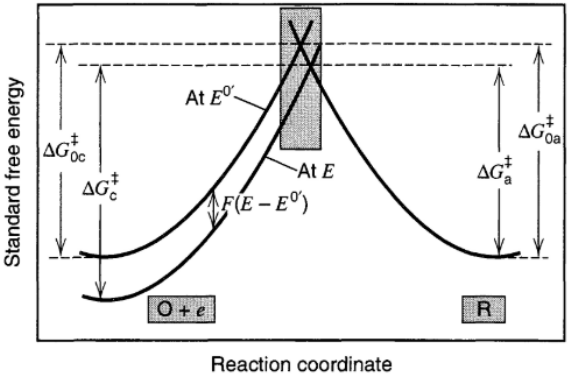
\includegraphics[width=0.45\textwidth]{Immagini/ButlerVolmer.png}
    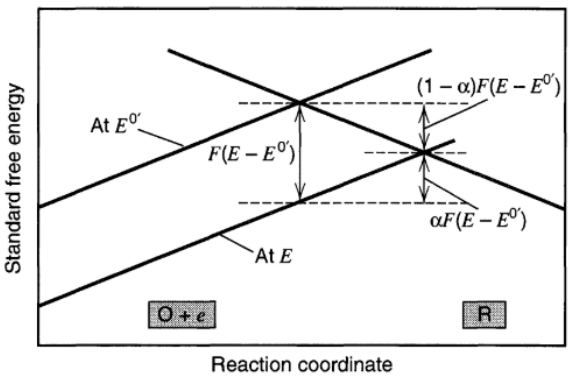
\includegraphics[width=0.45\textwidth]{Immagini/ButlerVolmer2.png}
    \caption{
        Approximation of the potential energy landscape inside a general reaction for some reaction coordinates. We are basically assuming that the reactants and products are minima in the energy and approximating the surrounding potential using second order Taylor expansion, so that the potential barrier is given by the interception of the parabolas.
    }
    \label{fig:ButlerVolmer}
\end{figure}
In that figure two conditions are depicted, a first one where we are in equilibrium so that the minima sits at the same height having so the same $\Delta G^\ddagger$ and therefore same rate, leading to $J = 0$. Then, we have the case where an external bias is applied and the energy of the electrons falls setting the reactants at lower potential generating a variation in the forward and backward barriers that can be estimated as follows
\begin{align*}
    &\Delta G_c^\ddagger = \Delta G_{0,c}^\ddagger - \alpha F(E - E^0), &\Delta G_a^\ddagger = \Delta G_{0,a}^\ddagger + (1 - \alpha) F(E - E^0).
\end{align*} 
Where $\alpha$ can be seen as an asymmetric factor, called transfer coefficient, that can range from zero to unity. Using these relations allows us to write down a form for the rates by inserting them inside \eqref{eq:transitionRate} to obtain
\begin{align}
    \label{eq:forwardRateC}
    &k_c = \kappa\frac{k_BT}{h}e^{-\frac{\Delta G^\ddagger_{0,c}}{RT}}\exp\left( -\frac{\alpha F(E-E^0)}{RT} \right), \\
    \label{eq:BackwardRateB}
    &k_a = \kappa\frac{k_BT}{h}e^{-\frac{\Delta G^\ddagger_{0,a}}{RT}}\exp\left( -\frac{(\alpha -1)F(E-E^0)}{RT} \right).
\end{align}
Knowing all of that we are able to obtain a really important result that is able to tell us the entity of the current inside our system as follows.
\thm{Butler-Volmer equation}
{
    The current flowing through the interface of an electrode, performing a general redox reaction, inside a well stirred solution is given by the equation
    \begin{equation}
        i = i_0\left[ e^{-\alpha\frac{F\eta}{RT}} - e^{-(\alpha - 1)\frac{F\eta}{RT}} \right].
    \end{equation}
    Where $i_0$ is the equilibrium current at the cathode and anode, while $\eta$ measure the bias applied as the difference between the cell potential and the standard one.
}
\pf{Proof}
{
    From \eqref{eq:forwardRateC} and \eqref{eq:BackwardRateB} we can see how, since the system was supposed to be in equilibrium without bias, meaning $E=E^0$, the rates have the properties of $k_c(E=0) = k_b(E=0)$. This brings us to write down that
    \begin{equation}
        k^0 = \kappa\frac{k_BT}{h}e^{-\frac{\Delta G^\ddagger_{0,c}}{RT}} = \kappa\frac{k_BT}{h}e^{-\frac{\Delta G^\ddagger_{0,a}}{RT}},
    \end{equation}
    which substituted back into the equation and inserted inside \eqref{eq:TotalCurrentInterface} gives the result
    \begin{equation}
        i = FAk^0\left[ C_O(0,t)e^{-\alpha\frac{F(E - E^0)}{RT}} - C_R(0,t)e^{-(\alpha - 1)\frac{F(E-E^0)}{RT}} \right].
    \end{equation}
    Now, in the equilibrium we have that $i = 0$ meaning how $i_c = i_a = i_0$ taking the name of \textbf{exchange current}, which can be found out easily from previous equation. In fact, by assuming equilibrium mass transfer is much faster than charge one surface concentration in electrode is equal to bulk one $C_0(0, t) = C_{O,b}$, so that we can write down
    \begin{equation}
        i_0  = FAk^0c_{O,b} e^{-\alpha\frac{F(E_{eq}-E^0)}{RT}}.
    \end{equation} 
    Since the system is at equilibrium we can use also Nernst equation in order to express the value of $E_{eq}$ as a function of concentration so that we can rewrite $i_0$ as
    \begin{align}
        &\frac{C_{O,b}}{C_{R,b}} = \exp\left[ \frac{F}{RT}(E_{eq} - E_0) \right], & i_0 = FAk^0 C_O^{1-\alpha}C_R^\alpha.
    \end{align}
    Inserting it inside the previous equation of $i$ and defining the \textbf{overpotential} $\eta$ as the difference $E - E_0$
    \begin{equation}
        i = i_0\left[ \frac{C_O(0, t)}{C_{O,b}} e^{-\alpha\frac{F\eta}{RT}} - \frac{C_O(0, t)}{C_{O,b}} e^{-(1-\alpha)\frac{F\eta}{RT}} \right],
    \end{equation}
    then in a stirred solution we also can assume that the surface concentration is equal to bulk one even out of equilibrium having that the fracions simplifies obtaining the right equation wanted.
}
\noindent
This equation is the key to understand how we can act on the variables of the system in order to boost the kinetics of the reaction. In particular, we can see how increasing both the external bias or the temperature can have huge effect on the reaction itself due to the exponential dependence. Also, one can see how the value of the exchange current posses a really important role since 
\begin{figure}[t]
    \centering
    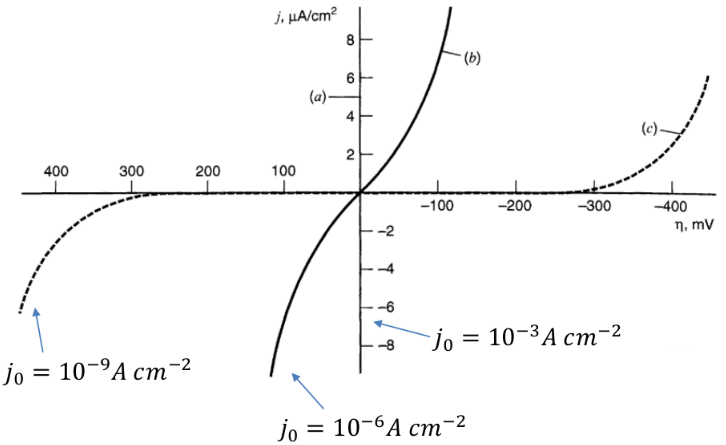
\includegraphics[width=0.8\textwidth]{Immagini/CurrentTrans.png}
    \caption{
        Graphic of the net current inside the cell as a function of the overpotential for different values of the exchange current, showing how the value of $i_0$ gives a great contribution to the overall current.
    }
    \label{eq:CurrentTrans}
\end{figure}
we can see from \figref{eq:CurrentTrans} how a lower $i_0$ gives a more \textbf{sluggish kinetics}. Where, a kinetics is more sluggish if you need a higher potential in order to obtain any net current at all inside the system.

Knowing such form for the current we can use it in order to perform some interesting computations regarding the kinetics properties. In particular, we can extract information about $\alpha$ and $i_0$ thanks to low and large $\eta$ regime. In the former case we have that a Taylor expansion leads us to the linear form
\begin{align}
    &i = -R_{ct}\eta, &R_{ct} = \frac{i_0 F}{RT},
\end{align}
the resistance $R_{ct}$ is called \textbf{charge-transfer resistance} and represent the impedance to charge transport intrinsic in the solution. Then, we can look at the case where $\eta \gg 1$, so that one of the two terms in the Butler-Volmer equation dominate so that we can easily write down
\begin{align}
    &i = i_0 e^{-\alpha \frac{F\eta}{RT}}, &\eta = \frac{RT}{\alpha F} \ln i_0 - \frac{RT}{\alpha F}\ln i.
\end{align}
Therefore, the potential linearly depends on the logarithm of the current giving rise to the form $\eta = a + b \ln i$ also called \textbf{Tafel theory}. The two constants inside such equation can be obtained with ease in experiments allowing us to estimate the values of both $\alpha$ and $i_0$.

\subsection{Mass transfer kinetics}

Butler-Volmer model allowed us to see how the kinetics of the system depends also on the surface concentration at the electrodes $C_i(0,t)$, which changes over time due to mass transport inside the material. Thus, we can't limit ourselves to the simple study of charge transport but to obtain a satisfying result we shall account also for the mechanisms of migration, convection and diffusion of material that can limit the flux of ions in the cell. In order to create such a model we are going to suppose to work in Nernstian conditions, so that equilibrium is present and the potential is given by Nernst equation, and we will also assume that the reaction is governed mass transport. Meaning that the rate at which the electroactive species is brought to the surface defines the current density
\begin{equation}
    J = nF\nu_{nt},
\end{equation}
where $\nu_{nt}$ is the flux of matter inside the electrolyte. Nevertheless, that is only the beginning of the model what we need to do now is to find out a more precise way to describe it.

The best way to model the flux of particle we can use a general form given by the sum of the contribution given by the three main processes mentioned before
\begin{equation}
    \nu_i(x) = -D_i\pdv{c_i}{x} - \frac{z_i F}{RT}D_i c_i\pdv{\Phi}{x} + c_iv(x).
\end{equation}
Where we have, in order, diffusion, migration and convection contribution, and $v$ represent the velocity of the solution in a certain point. Obviously such an equation is really complex, therefore we usually need to simplify it by setting ourselves in a situation where one or two contributions can be neglected such as:
\begin{itemize}[align=left, leftmargin=*]
    \item[\textbf{Diffusion.}] Introducing stirring;
    \item[\textbf{Migration.}] Addition of a concentrated supporting electrolyte;
    \item[\textbf{Convection.}] Avoiding vibrations or stirring. 
\end{itemize}
Therefore, we can choose to use one or more trick in order to eliminate the related processes. Thus, we are going to imagine to work in a diffusion limited process so that $\nu_i$ is defined simply by Fick's first law and the current density becomes
\begin{equation}
    J = nF\nu_d = nFD\eval{\dv{C_O}{x}}_{x=0}.
\end{equation} 
Where the derivative is evaluated at the interface and in a stirred solution we can assume that the bulk concentration is stable in the middle of the solution, meaning that $C_O$ is constant at $C_{O,b}$ for $x$ large enough. In this way we can approximate the derivative simply as a difference of the kind
\begin{equation}
    \label{eq:CurrentDiffusion}
    J \approx nFD\frac{C_{O,b} - C_{O}(x=0)}{\delta},
\end{equation}
where $\delta$ is a constant that needs to be tuned in order to optimize the approximation called \textbf{Nernst Diffusion Layer thickness} and can be seen in \figref{fig:ApproxDensGrad}.
\begin{figure}[t]
    \centering
    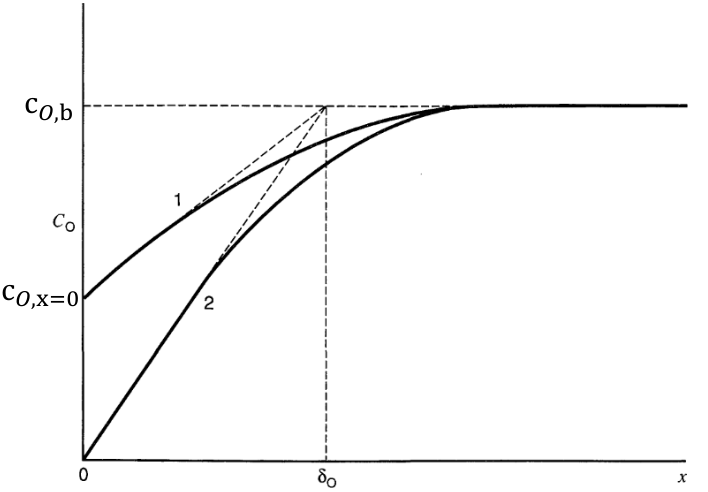
\includegraphics[width=0.8\textwidth]{Immagini/ApproxDensGrad.png}
    \caption{
        Representation of the concentration gradient approximation to understand what $\delta$ effectively looks like and how the concentration is.
    }
    \label{fig:ApproxDensGrad}
\end{figure}
From that we can see how the diffusion is quicker the smaller $\delta$ is or the more negative the potential becomes. Still, it's quite difficult to know the value of $\delta$ so that it's value is usually combined with the diffusivity defining the \textbf{mass-transfer coefficient} $m_i = D_i/\delta_i$. This relation can be used in order to describe the limiting behavior that the mass transport has on the kinetics of the reaction by seeing the following result.
\thm{Limiting current}
{
    Inside an electrochemical cell where mass transport is driven by diffusion the system posses a limiting current given by
    \begin{equation}
        \label{eq:LimitingCurrent}
        J_L = nFm_O C_{O,b}.
    \end{equation}
}
\pf{Proof}
{
    Since electrons travels at higher speeds respect to diffusion of ions in the solution, the rate of the reaction is limited for high value of the overpotential by the maximum flux of ions possible in the electrolyte. In particular, we have seen how \eqref{eq:CurrentDiffusion} gives a way to estimate the rates inside the system for both O and R transfer, where the latter can be expressed by changing the constants and remembering how the electrode is positioned on the right and the solution on the left, so you need to invert the concentrations
    \begin{equation}
        \label{eq:CurrentGen}
        J = nFm_R (C_{R, x=0} - C_{R,b}).
    \end{equation} 
    In both equations we can see how the maximum possible value that we can obtain is when the density of element on the surface of the electrode is zero, $C_{O, x=0} = 0$. That is the maximum flux that we can obtain, giving rise also to the maximum possible current inside the system.
}
\noindent
This relation can also be used in order to rewrite the concentrations of the elements in the solution in a simpler way. In particular, if you use the previous relation alongside with the form of the limiting current we can obtain that
\begin{align}
    \label{eq:OssConcentration}
    &C_{O}(x=0) = \frac{J_L - J}{nFm_O}, &\frac{C_{O}(x=0)}{C_{O, b}} = 1 - \frac{J}{J_L},
\end{align}
which will be really useful in further descriptions. In particular, using such relations one can see how a value for the cell potential can be found out by assuming how the initial concentration of reduced specie is zero $C_{R,b} = 0$. This assumption inserted inside \eqref{eq:CurrentGen} allows us to obtain $C_{R, x=0} = J/nFm_R$ which inserted inside Nernst equation, alongside with \eqref{eq:OssConcentration}, to obtain
\begin{equation}
    E = E^0 - \frac{RT}{nF}\ln\frac{m_O}{m_R} + \frac{RT}{nF}\ln\left( \frac{J_L - J}{J} \right).
\end{equation}
Such equation shows interesting behavior since all the quantities inside it are easy to evaluate experimentally, still only works if at the start of the reaction only one element is present in the solution. Nevertheless, we can see how at a certain value of the current $J = J_L/2$ the equation simplifies a lot, having
\begin{equation}
    E_{1/2} = E^0 - \frac{RT}{nF}\ln\frac{m_O}{m_R},
\end{equation}
which value is often taken equal to $E^0$ since $m_O/m_R \approx 1$ in most of the cases. Therefore, that value is often used in order to rewrite the total equation substituting it, giving the final general form of the equation
\begin{equation}
    E = E_{1/2} + \frac{RT}{nF}\ln\left( \frac{J_L - J}{J} \right).
\end{equation}
In reality is possible to describe a model also for the case where both reduced and oxidized species are present inside the solution at time zero. In that case is important to take into account that two different limiting currents are present inside the material, one in the cathodic and one in the anodic direction as
\begin{align}
    &J_{L,c} = nFm_OC_{O,b}, &J_{L,a} = -nFm_RC_{R,b}.
\end{align}
Which comes out from the same theory used previously to find \eqref{eq:LimitingCurrent}, meaning that the relations \eqref{eq:OssConcentration} are valid also for $C_R$. In this way we can substitute everything inside the Nernst equation to gain the final general result
\begin{equation}
    E = E^0 - \frac{RT}{nF}\ln\frac{m_O}{m_R} +\frac{RT}{nF}\ln\left( \frac{J_{L,c} - J}{J - J_{L,a}} \right).
\end{equation}
This is a more general result that can be used, which also posses a peculiar property. In fact, is possible to see by this equation how the potential at equilibrium, $J=0$, gives out exactly Nernst equation $E^0 + RT\ln(C_{O,b}/C_{R,b})/nF$.

All of this theory is great but is only an approximation frozen in time to estimate the limiting current. In reality, the value of $J_L$ can change overtime due to changes in the concentration of the species inside the solution, but more importantly by the variation of the concentration gradient inside it due to diffusion processes. In particular, we can describe such a process by using the following result.
\thm{Cottrell equation}
{
    If the reaction is Nernstian the limit current density decreases with time, following the equation
    \begin{equation}
        \label{eq:TimeDepLimitingCurrent}
        J_L = nFC_{O,b}\sqrt{\frac{D}{\pi t}}.
    \end{equation}
}
\pf{Proof}
{
    If the reaction is Nernstian, the concentration at the electrode surface immediately adjusts to the equilibrium value, but its gradient slowly shifts due to diffusion. The thickness of the Nernst diffusion layer is then time-dependent
    \begin{equation}
        \delta(t) = \sqrt{\pi Dt},
    \end{equation}
    which can be substituted inside \eqref{eq:CurrentDiffusion} to obtain the result. Inside it, we assume $C_{O,b}$ is constant in time since if the solution is stirred it gets homogeneous in the bulk really quickly, the problem is only the gradient at the boundary.
}
\nt
{
    As it was sad the presence of convection allows us to assume $C_{O,b}$ constant over time inside \eqref{eq:TimeDepLimitingCurrent}, but it also generates one other thing. Basically, since the bulk concentration is homogeneous, the presence of convection is also limiting the diffusion in decreasing the gradient, meaning that when it is flattened to a certain point it can go any further since it needs to change the part of solution that has constant concentration thanks to convection. For this reason, in presence of convection $J_L(t)$ will not decrease indefinitely with time, but will reach a plateu.
}

\subsection{Microscopic theories for charge transfer}

So far so good, nevertheless all the theory described right now are of a phenomenological type, focussing on describing the phenomena using a series of constant that we need to compute experimentally, like $k^0$ or $\alpha$. Now we want to relax such condition creating a more fundamental model for charge transfer inside the solution that can limit the number of constant that we are using. Thus, we are going to describe a famous model called \textbf{Marcus model} which is able to find a form of the transition rate dependent only on one phenomenological constant that can be also modelled via first principles.

We are interested in study the exchange of one electron from the electrode, so a metal, to the oxidation molecule inside the solution. The latter, is going to be modelled as a metallic sphere with a certain dipole and dielectric constant, which can interact with the electrode in two main ways: \textbf{outer sphare}, where the molecule is separated from the surface by a layer of solvent so that the $e^-$ needs to travel by tunneling effect, or \textbf{inner sphere}, where a strong interaction is present so that the molecule is close to the surface leading to the exchange. We are not going to pick one of the two cases, since both will be described by the model, as we will see, which simply focus on the transfer of the charge making the following four assumptions:
\begin{itemize}[align=left, leftmargin=*]
    \item[\textbf{Isoenergetic process.}] the electron must move from an initial state (on the electrode or in the reductant, R) to a receiving state (in species O or on the electrode) of the same energy;
    \item[\textbf{Franck-Condon.}] Basically no change in the atomic configuration happens, meaning that the nuclei remains still since electronic processes are much faster respect to atomic ones;
    \item[\textbf{Fixed position.}] The reactant O has fixed position with respect to the electrode;
    \item[\textbf{Quadratic $G$.}] Standard free energies of O and R, $G_O$ and $G_R$, depend quadratically on the reaction coordinate, $q$. 
\end{itemize}
Keeping in mind such approximations we are able to find out a general way to write down the transition rate for the reaction in general as follows.
\thm{Marcus result}
{
    Inside an electrochemical cell where the four conditions before mentioned are satisfied, the transition rate for the charge transfer process is given by
    \begin{equation}
        k = \kappa Z \exp\left[ -\frac{\lambda}{4RT}\left( 1 + \frac{\Delta G^0}{\lambda} \right)^2  \right],
    \end{equation}
    where $\kappa$ is usually taken as $1$, $Z$ is a function of an electrostatic and collisional term, and $\lambda$ is the so-called reorganization energy accounting for both inner and outer interactions.
}
\pf{Proof}
{
    the free energy is approximated to a quadratic form, therefore we can write down
    \begin{align}
        &G_O(q) = \frac{k}{2}(q-q_O)^2, &G_R(q) = \frac{k}{2}(q - q_R)^2 + \Delta G^0,
    \end{align}
    where $k$ is a proportionality constant and $\Delta G^0$ is the usual potential bias $F(E-E^0)$. Having both this values we can put them in a system and find out the point where the two curves intersect giving rise to the approximated transition state. Such a computation gives rise to the result
    \begin{align}
        q^\ddagger = \frac{q_R + q_O}{2} + \frac{\Delta G^0}{k(q_R - q_O)},
    \end{align}
    which can be used in order to evaluate the potential barrier for the oxidation process as $G_O(q^\ddagger) - G_O(q_O)$ which gives rise to
    \begin{equation}
        \Delta G^\ddagger = \frac{k(q_R - q_O)^2}{8}\left[ 1 + \frac{2\Delta G^0}{k(q_R - q_O)^2} \right]^2 = \frac{\lambda}{4}\left[ 1 + \frac{\Delta G^0}{\lambda} \right]^2.
    \end{equation}
    \begin{figure}[t]
        \centering
        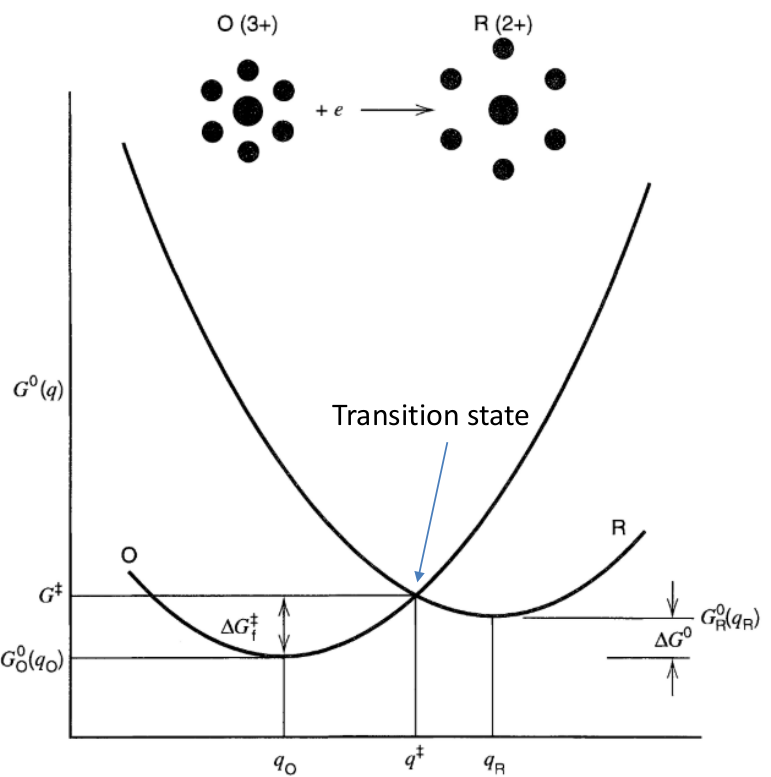
\includegraphics[width=0.37\textwidth]{Immagini/MarcusApprox.png}
        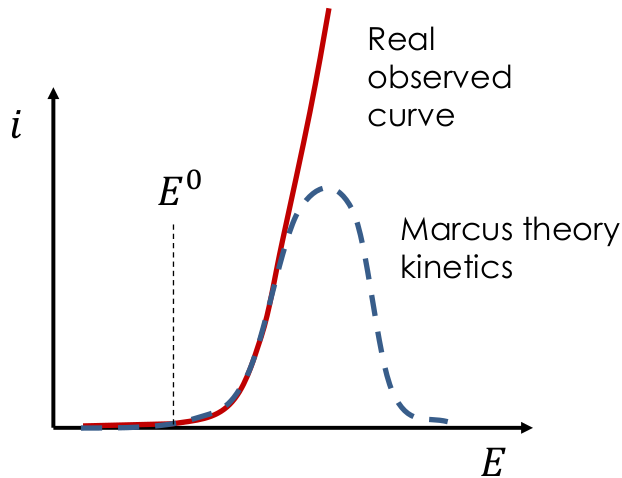
\includegraphics[width=0.5\textwidth]{Immagini/MarcusRes.png}
        \caption{
            Representation of the energy landscape of the reaction in the Marcus approximation, on the left, and the graph of the result model obtained versus the experimental result, on the right.
        }
    \end{figure}
    Therefore, we have a form for the potential barrier which depends on the form of the reorganization energy. The latter can be evaluated by taking into account the inner and outer components' contribution to the reorganization of the species O and the solvent $\lambda = \lambda_i + \lambda_o$. Both of them can be modelled, the latter is given by the sum of normal vibration modes of reactants
    \begin{equation}
        \lambda_i = \sum_j \frac{k_j}{2}(q_{O,j} - q_{R,j})^2.
    \end{equation}
    The latter, instead, is computed by calculating the ion-solvent electrostatic interaction for reactant and products, assuming the solvent as a dielectric continuum and the reactant a sphere of radius $a_O$
    \begin{equation}
        \lambda_o = \frac{e^2}{8\pi\varepsilon_0} \left( \frac{1}{a_O} - \frac{1}{R} \right)\left( \frac{1}{\varepsilon_{op}} - \frac{1}{\varepsilon_s} \right).
    \end{equation}
    Where $R$ is twice the distance of molecule and surface of electrode, while the dielectric constants are the one of the molecule and of the electrode. Knowing this we can insert that value inside the known form of the transition rate in order to obtain the wanted relation.
}
\noindent
This model is really great, showing how depending on the ratio $\Delta G^0/\lambda$ the reaction will actually change its velocity. In particular, we can see how for biases so that $\Delta G^0 < -\lambda$ we got $k \propto \Delta G^0$ reaching a maximum in $\Delta G^0 = -\lambda$ and then having $k \propto 1/\Delta G^0$ for higher values. This is a really strange behavior since experimentally the so-called \textbf{inverted region} is not seen, as we increase the potential the reaction speeds up and that was the reason because the model took some time to be accepted by the community. The reason why this happens are basically two: the first is that \textbf{O are not still}, basically as $E$ is increase the molecule interact more with the electrode lowering the distance $R$ and so increasing $\lambda$, and \textbf{More levels are involved}, the model we have described assumed that the electron transferred is taken from the higher level inside the electrode, the Fermi level, that is true only in practice since as we increase the potential the electrons in lower levels can be exited and transferred too. 

This theory can be in principle expanded in order to account better for such effect in a higher approximation by using the \textbf{Gerischer-Marcus model}. The latter uses the assumption that electrons are able to jump only from one occupied state into an unoccupied isoenergetic state, where the occupied state for a reduction is inside the metal electrode and the unoccupied is on species R in the solution, while for oxidation is the contrary. In this way the information we need in order to describe the evolution of the reaction are contained inside the DOS of the metal and of the reactant. In particular, in this case it's better to express the density of states inside the solution using a concentration of type $D_R(\lambda, E)\dd E$, giving the concentration of species R in the solution in the energy range $[E , E + \dd E]$. We expect such concentration to be somehow proportional to the surface concentration of R on the electrode, so that we will assume the possibility to rewrite it as
\begin{align}
    &D_R(\lambda, E) = N_A C_R(0, t) W_R(\lambda, E), & \int_\mathbb{R}W_R(\lambda, E)\dd E = 1.
\end{align}
\begin{figure}[t]
    \centering
    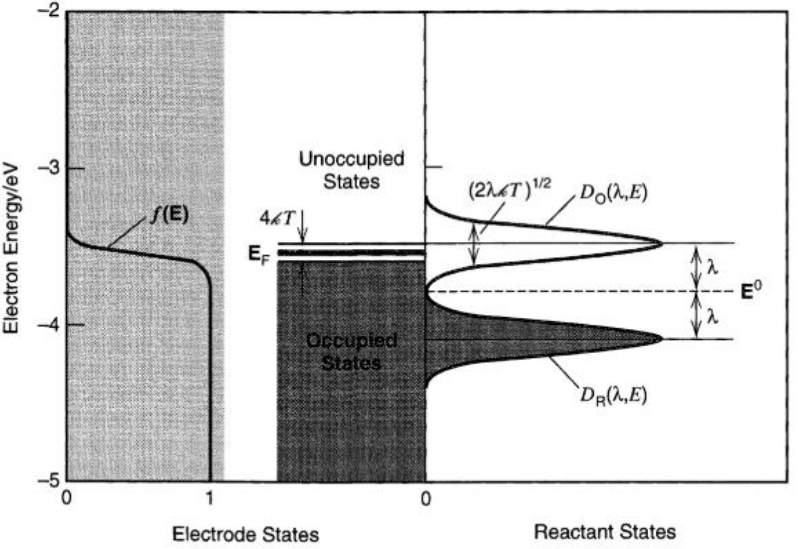
\includegraphics[width=0.8\textwidth]{Immagini/GMtheory.png}
    \caption{
        Example graph of the density of state of a metal near the concentration of the species energies, showing how the O states are able to overlap with occupied states, meaning that the integral for $k_f$ is not zero allowing for the reaction to happen.
    }
    \label{fig:GMtheory}
\end{figure}
Where the function $W_R(\lambda, E)$ can be thought of a probability density distribution of having the specie at that specific energy under the influence of that reorganization energy. Knowing this it's possible to obtain a result to describe the transitions rates for the oxidation and reduction reaction in terms of such functions as follows.
\thm{Transition rates}
{
    The transition rates inside the Gerischer-Marcus model can be computed as the following integrals
    \begin{align}
        &k_f = \nu\int_\mathbb{R} \varepsilon_{red}(E)W_O(\lambda, E) f(E)\rho(E)\dd E, &k_b = \nu\int_\mathbb{R} \varepsilon_{ox}(E)W_R(\lambda, E) [1-f(E)]\rho(E)\dd E.
    \end{align}
    Where $\varepsilon_{ox}$ and $\varepsilon_{red}$ are proportionality functions involving the tunneling probability and precursor equilibrium constants. Also, $\rho(E)$ and $f(E)$ are DOS and Fermi function of the metal.
}
\noindent
Using such results we are able to evaluate the transition rate in a general way, we only need to find out a way to model the probability density $W$. Such a task can be done by using once again the Marcus theory, which allows us to obtain the following forms
\begin{align}
    &W_O(\lambda, E) = \frac{1}{\sqrt{4\pi\lambda k_BT}}\exp\left[ -\frac{\left( E - E^0 - \lambda \right)^2}{4\lambda k_BT} \right], \\
    &W_R(\lambda, E) = \frac{1}{\sqrt{4\pi\lambda k_BT}}\exp\left[ -\frac{\left( E - E^0 + \lambda \right)^2}{4\lambda k_BT} \right].
\end{align}
Such results show also how the states of O and R species have peaks of densities specular to each others and the transition rates increase as such peaks come closer to point of high density of states inside the metal, as we can see in \figref{fig:GMtheory}. Therefore, based on the value of $\lambda$ and of the Fermi energy, $E_f$, we are able to change the overlap of the states increasing $k_f$ or $k_b$ as we want. In fact, the value of $E_f$ can be changed by an external bias, shifting it up and down the levels along with the direction of the reaction, as we have already seen previously.
\nt
{
    Such a theory is particular good in order to describe the effect of using electrodes made of semiconductor, since their behavior can be easily described by the simple use of a density of state with a gap in the middle.
}